\section{Sections fine tuning}

\paragraph{Second T}
Regarding the optimization of the second T junction we used the T designed for the previous assignment and we connect to it the two lines routing to the patches. In this way we control also the contributions due to the discontinuities on all the second part of the beam forming network.

Simulating this new component we have that the matching is no more on the wanted frequency of $2.45GHz$ but some megahertz higher. In order to make it decrease at first we tried to change the values external to the T junction with a freedom degree, that in particular are the angle and the tapering of the bending. The results varying those values are showed in the graphs below. Notice that in practice the resonance is not moved in both the cases.
\begin{figure}[H]
	\centering
	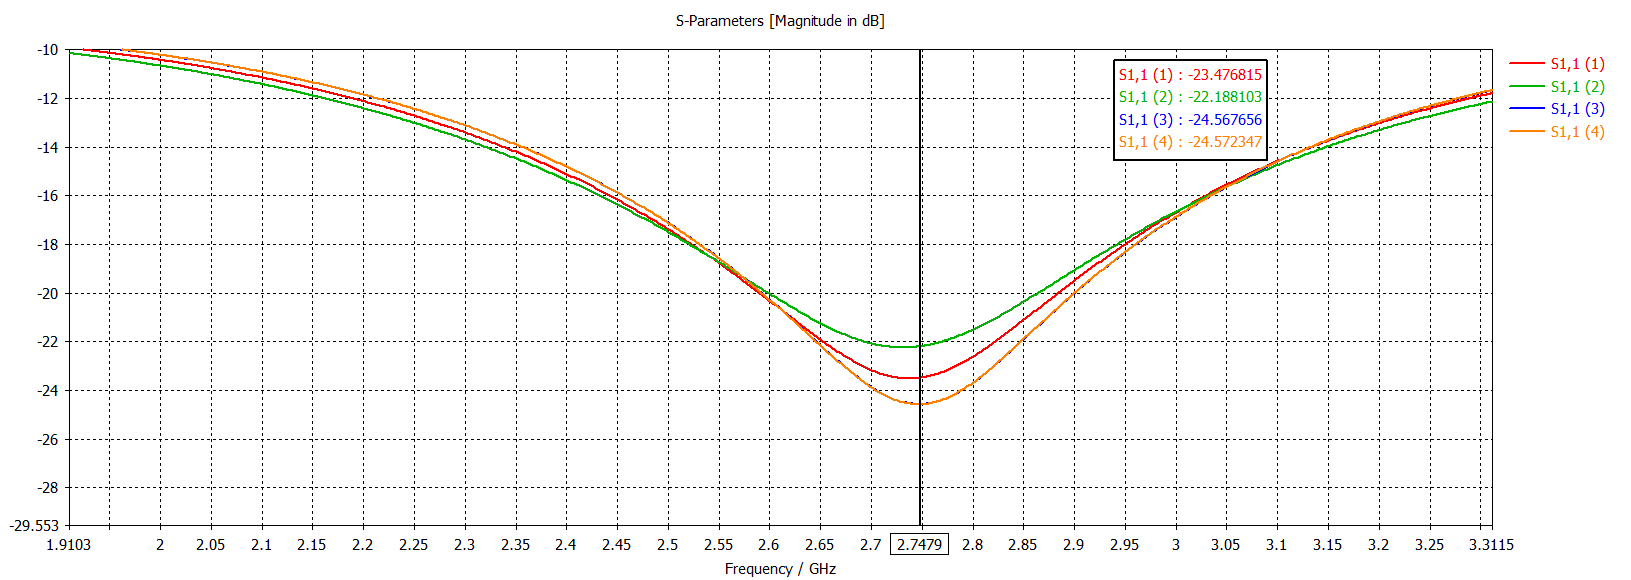
\includegraphics[width=1\linewidth]{sT_1angle.png}
	\caption{s11 with respect to the bend angle}
	\label{sT_1angle}
\end{figure}
\begin{figure}[H]
	\centering
	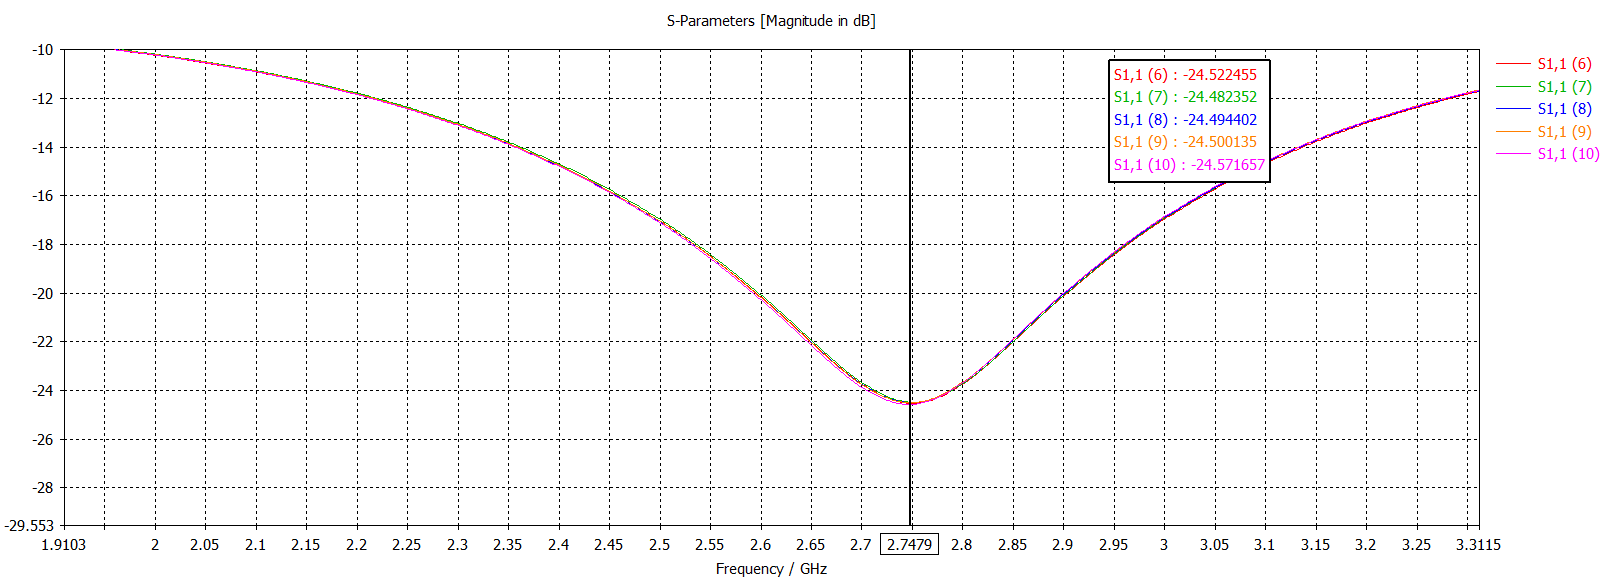
\includegraphics[width=1\linewidth]{sT_1depth.png}
	\caption{s11 with respect to the bend tapering}
	\label{sT_1depth}
\end{figure}
Now we have tried to not modify the T junction parameters, but since this way didn't produce the desired effect we have to change the the $\lambda/4$ impedance transformer's length. The graphs below shows the values obtained first with simply changing the transformer length and second the also re-using the old optimized value of the single T junction (notice that in the second case the return losses are lower).
%\begin{figure}[H]
%	\centering
%	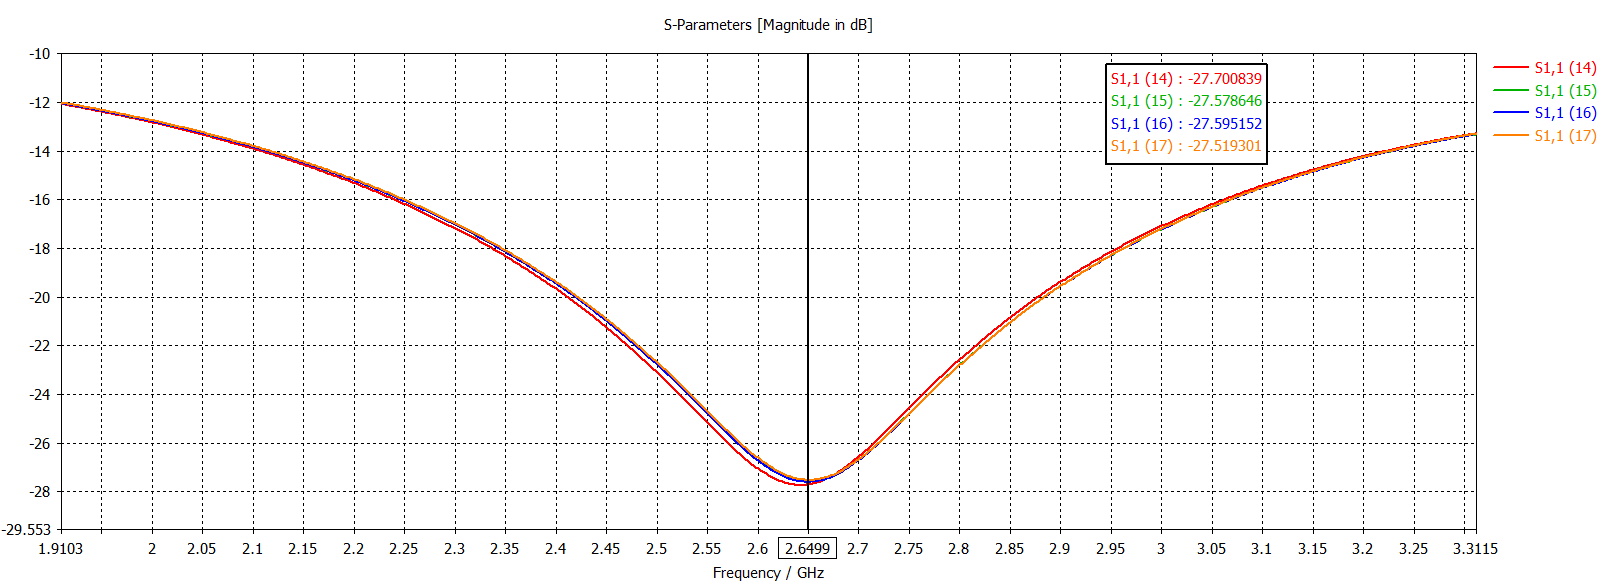
\includegraphics[width=1\linewidth]{sT_2depth.png}
%	\caption{}
%	\label{sT_2depth}
%\end{figure}
\begin{figure}[H]
	\centering
	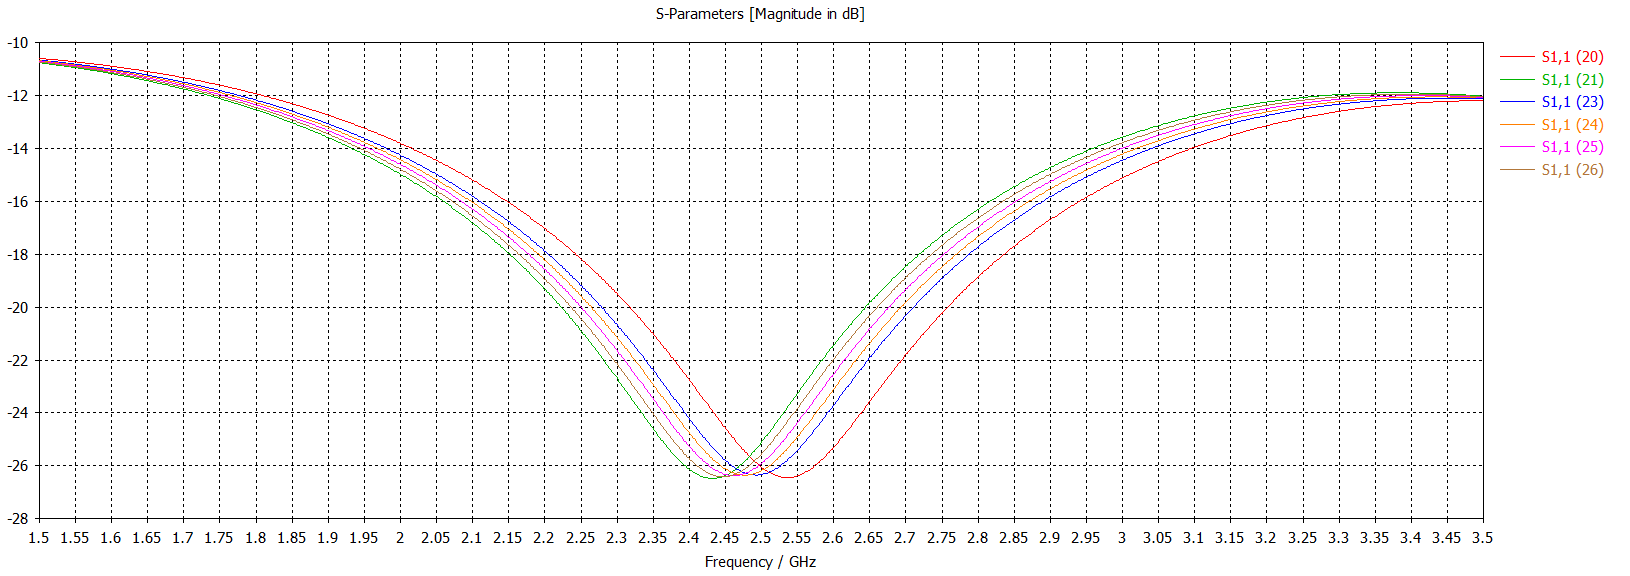
\includegraphics[width=1\linewidth]{sT_2par.png}
	\caption{s11 with respect to the $\lambda/4$ transformer's length}
	\label{sT_2par}
\end{figure}
\begin{figure}[H]
	\centering
	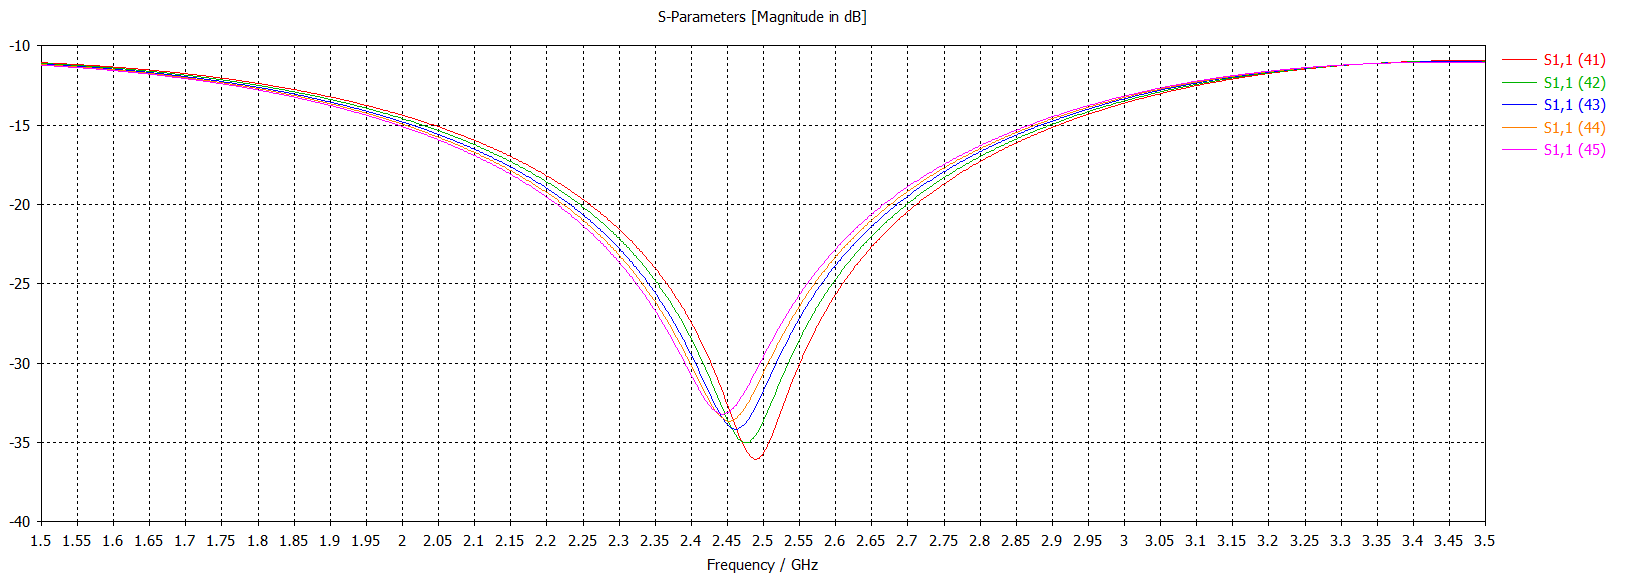
\includegraphics[width=1\linewidth]{sT_3par.png}
	\caption{s11 with respect to the $\lambda/4$ transformer's length -- changed values}
	\label{sT_3par}
\end{figure}
With this final value we reached the desired behavior, so we can use this for composing the complete beam forming network. On the following figure is showed the result, notice that also the $s_{21}$ and the $s_{31}$ have the proper values in order to generate the desired tapering.
\begin{figure}[H]
	\centering
	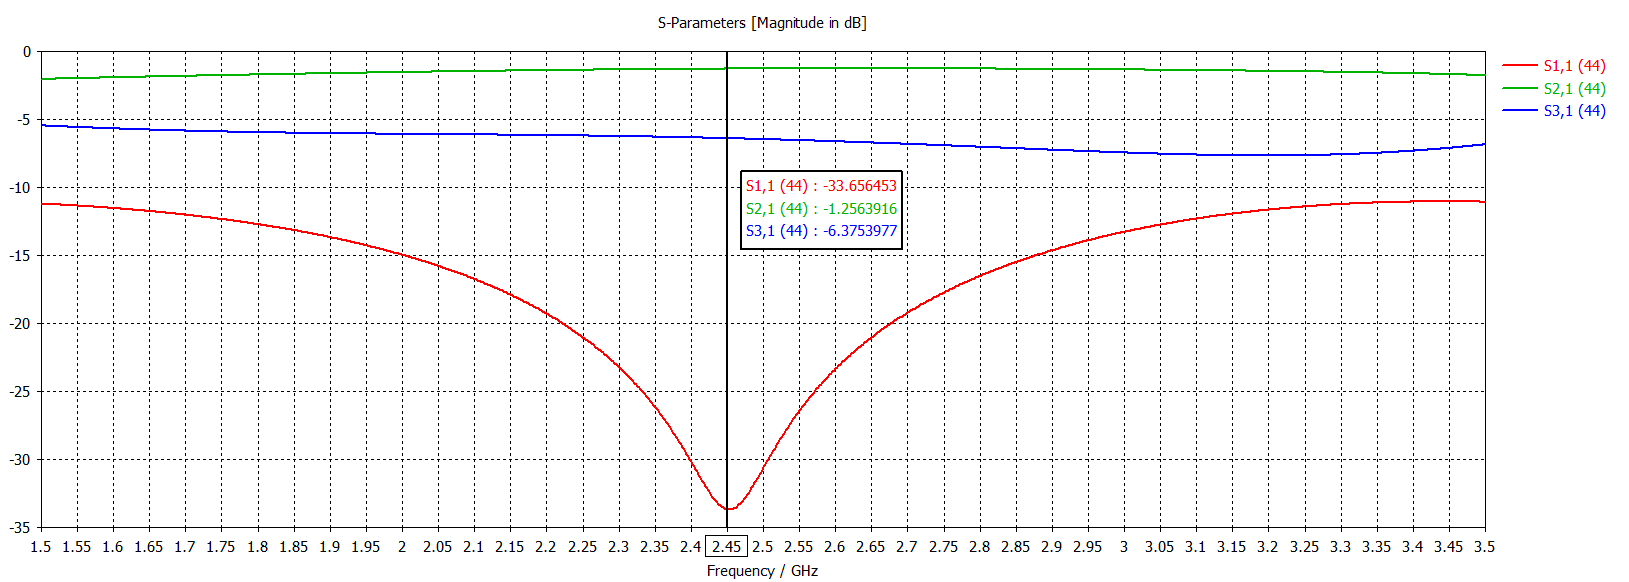
\includegraphics[width=1\linewidth]{sT_fin.png}
	\caption{}
	\label{sT_fin}
\end{figure}
